\section{Gesamtübersicht}\label{sec:gesamtubersicht}

Abbildung \ref{fig:results-evaluation-metrics-comparison} zeigt für jedes der untersuchten Modelle die durchschnittlichen Metrik-Werte über alle fünf Wiederholungen hinweg inklusive Standardabweichung. Für einen besseren Vergleich sind die proprietären Modelle rot, die kleineren Modelle orange und die größeren Modelle blau dargestellt. Diese Einteilung entspricht der in Kapitel \ref{ch:modellauswahl} beschriebenen Kategorisierung. Im folgenden wird zuerst ein Überblick über die Ergebnisse gegeben, bevor im Anschluss eine detaillierte Analyse erfolgt.

Positiv aufgefallen ist, dass neun von dreizehn Modellen das Qualitätsziel eines F1-Scores von $\geq 0{,}80$ erreichen konnten - darunter auch kleine Modelle. Dennoch übertreffen die großen Modell die Kleinen vor allem im F1-Score, was auf eine bessere Balance zwischen Präzision und Recall hindeutet. Über alle Metriken hinweg sind \texttt{Qwen3-235B-A22B-Thinking-2507}, \texttt{GPT-OSS-120B} und \texttt{GPT-OSS-20B} ganz vorne mit dabei. Auffällig ist das schwache Abschneiden des europäischen \texttt{Mistral-8x7B-Instruct-v0.1}-Modells, das sowohl in Precision, als auch Recall weit zurückfällt und als einziges Modell einen F1-Score von $\le 0{,}60$ erreicht.

\begin{figure}[htbp]
    \centering
    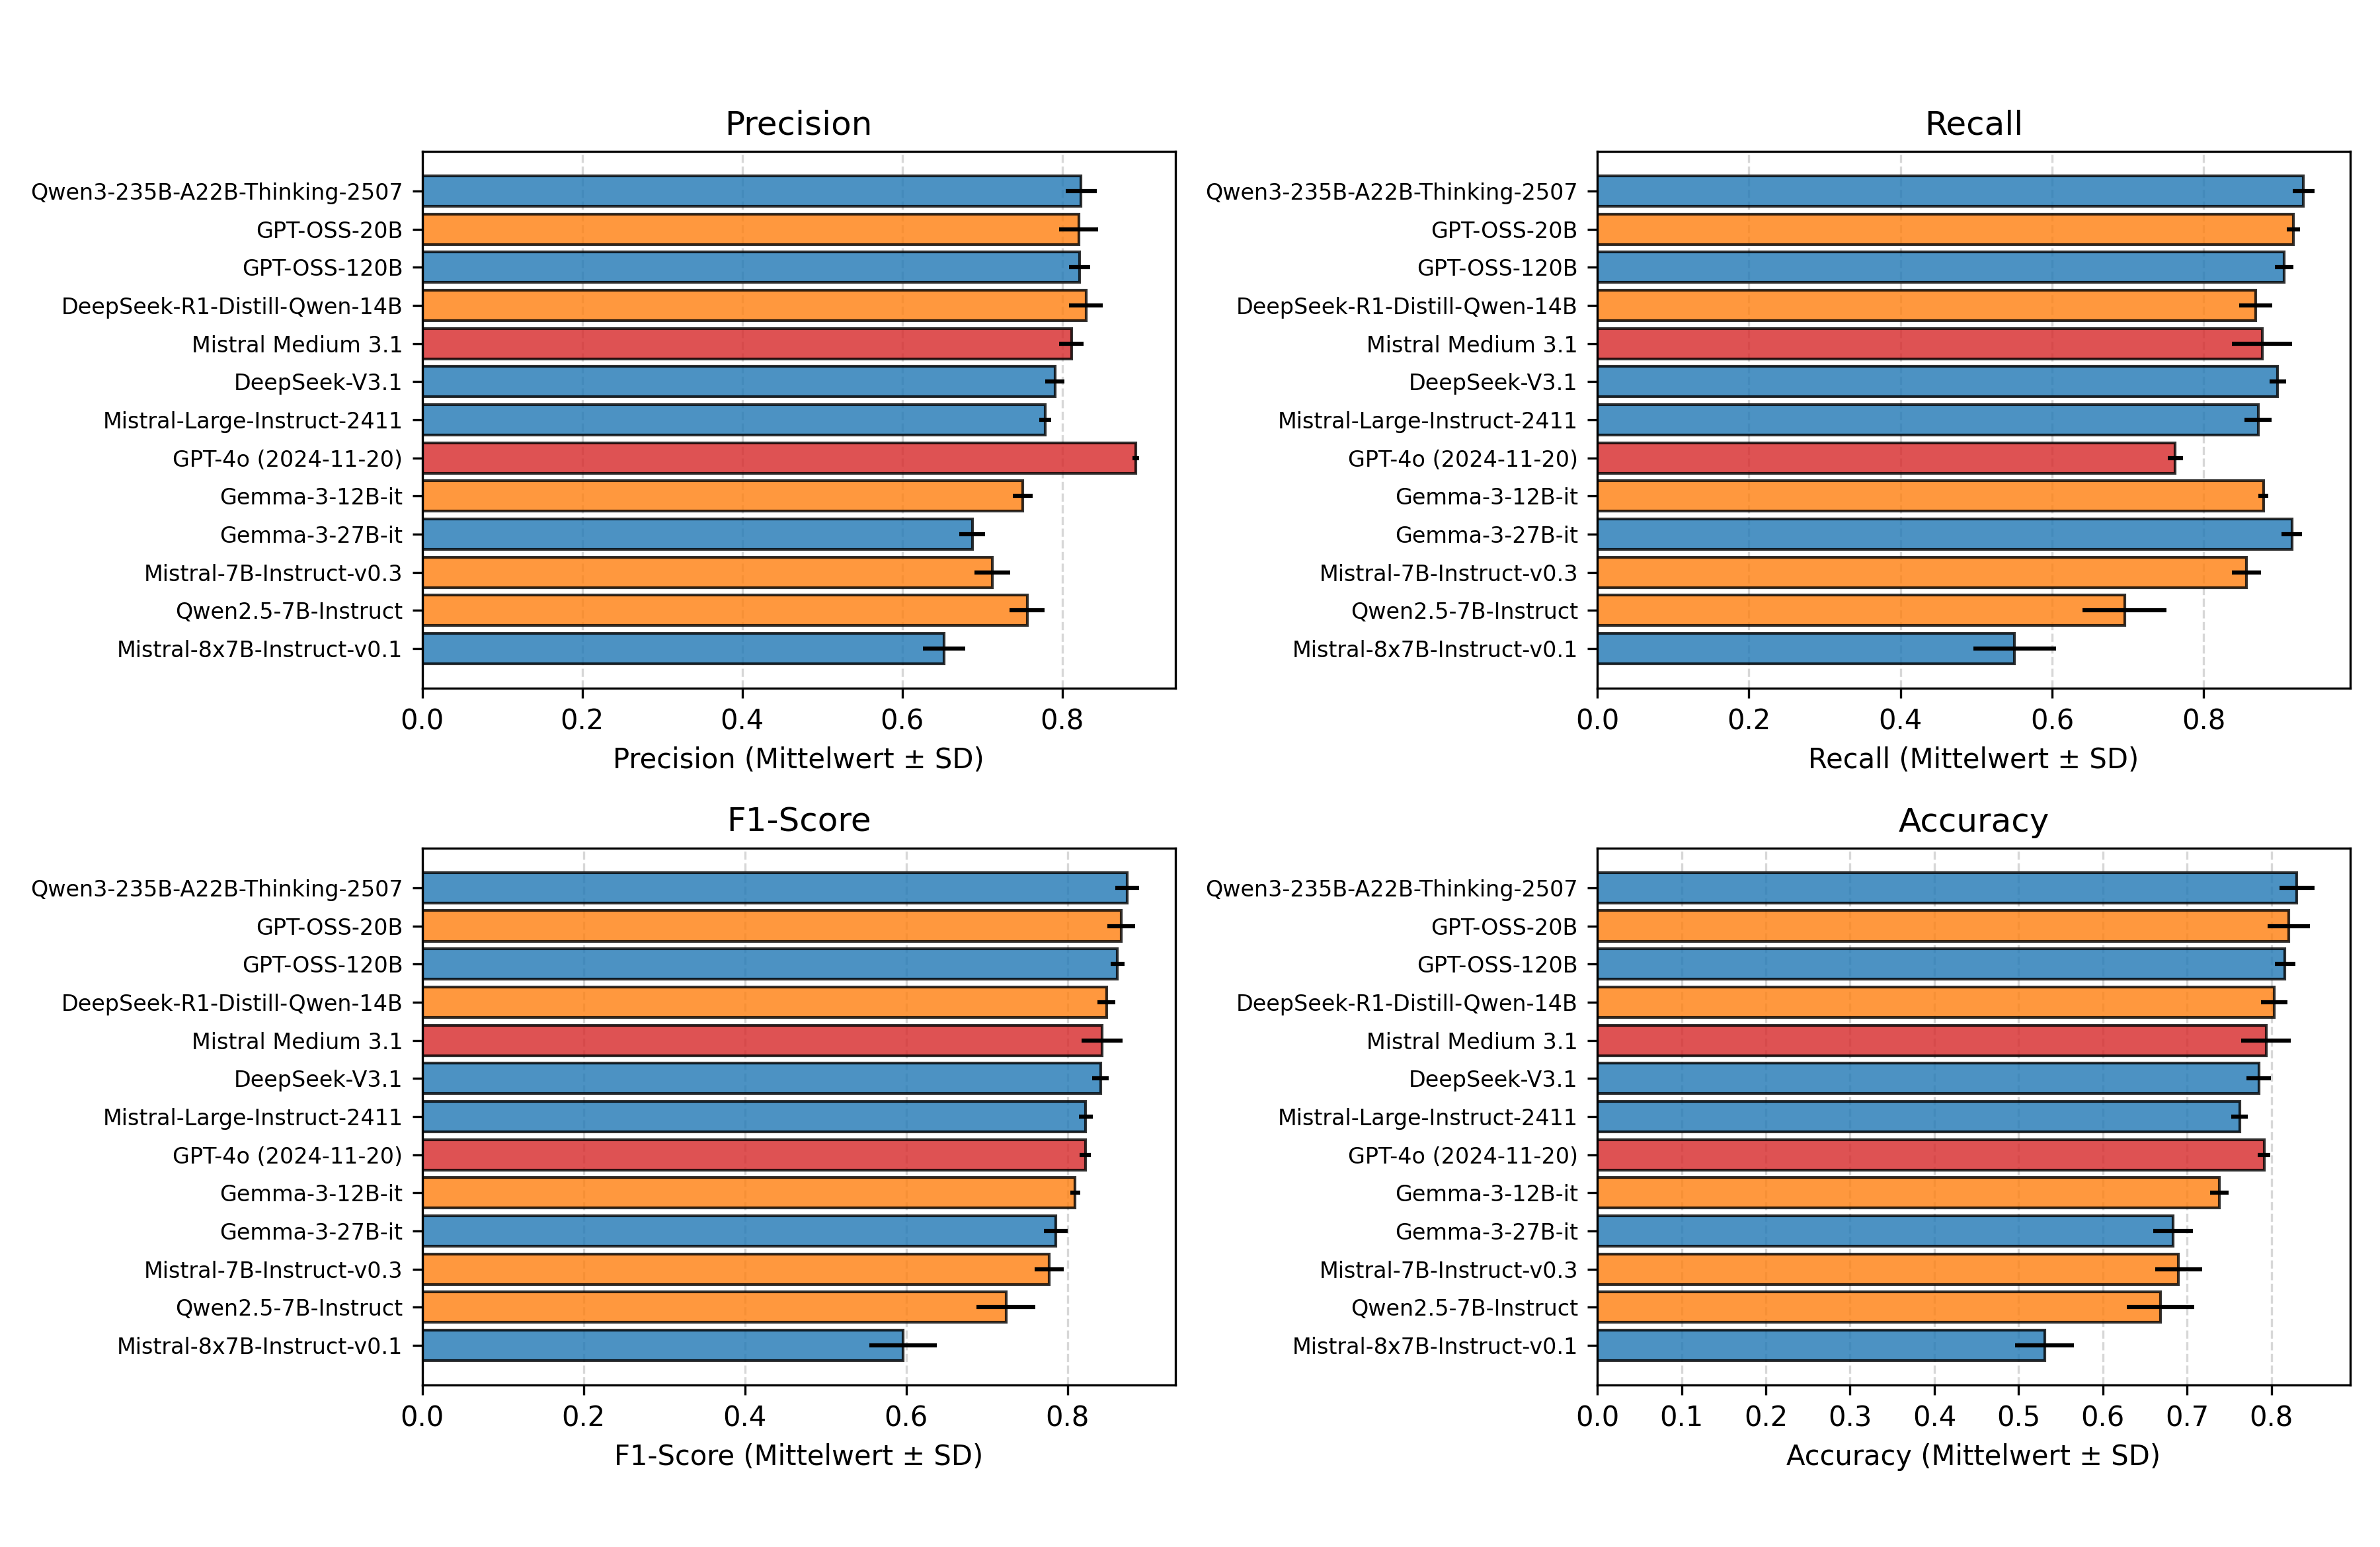
\includegraphics[width=\textwidth,trim=20 40 20 10,clip]{images/results/evaluation_metrics_comparison}
    \caption{Durchschnittliche Metrik-Werte der untersuchten Modelle über alle Wiederholungen hinweg inklusive Standardabweichung.}
    \label{fig:results-evaluation-metrics-comparison}
\end{figure}

Die Abbildung \ref{fig:results-evaluation-metrics-comparison} macht deutlich, dass einige Modelle – etwa \texttt{GPT-4o} oder\linebreak\texttt{Qwen-2.5-7B-Instruct} – hohe Präzisionswerte aufweisen, aber im Recall zurückliegen. Anders sieht es bei \texttt{Gemma-3-27B-it} aus, das einen sehr guten Recall erreicht, aber bei der Präzision auf dem vorletzten Platz liegt. Modelle wie \texttt{Qwen3-235B-A22B} und \texttt{GPT-OSS-20B} erreichen einen ausgezeichneten Recall bei gleichzeitig hoher Präzision.

\begin{figure}[htbp]
    \centering
    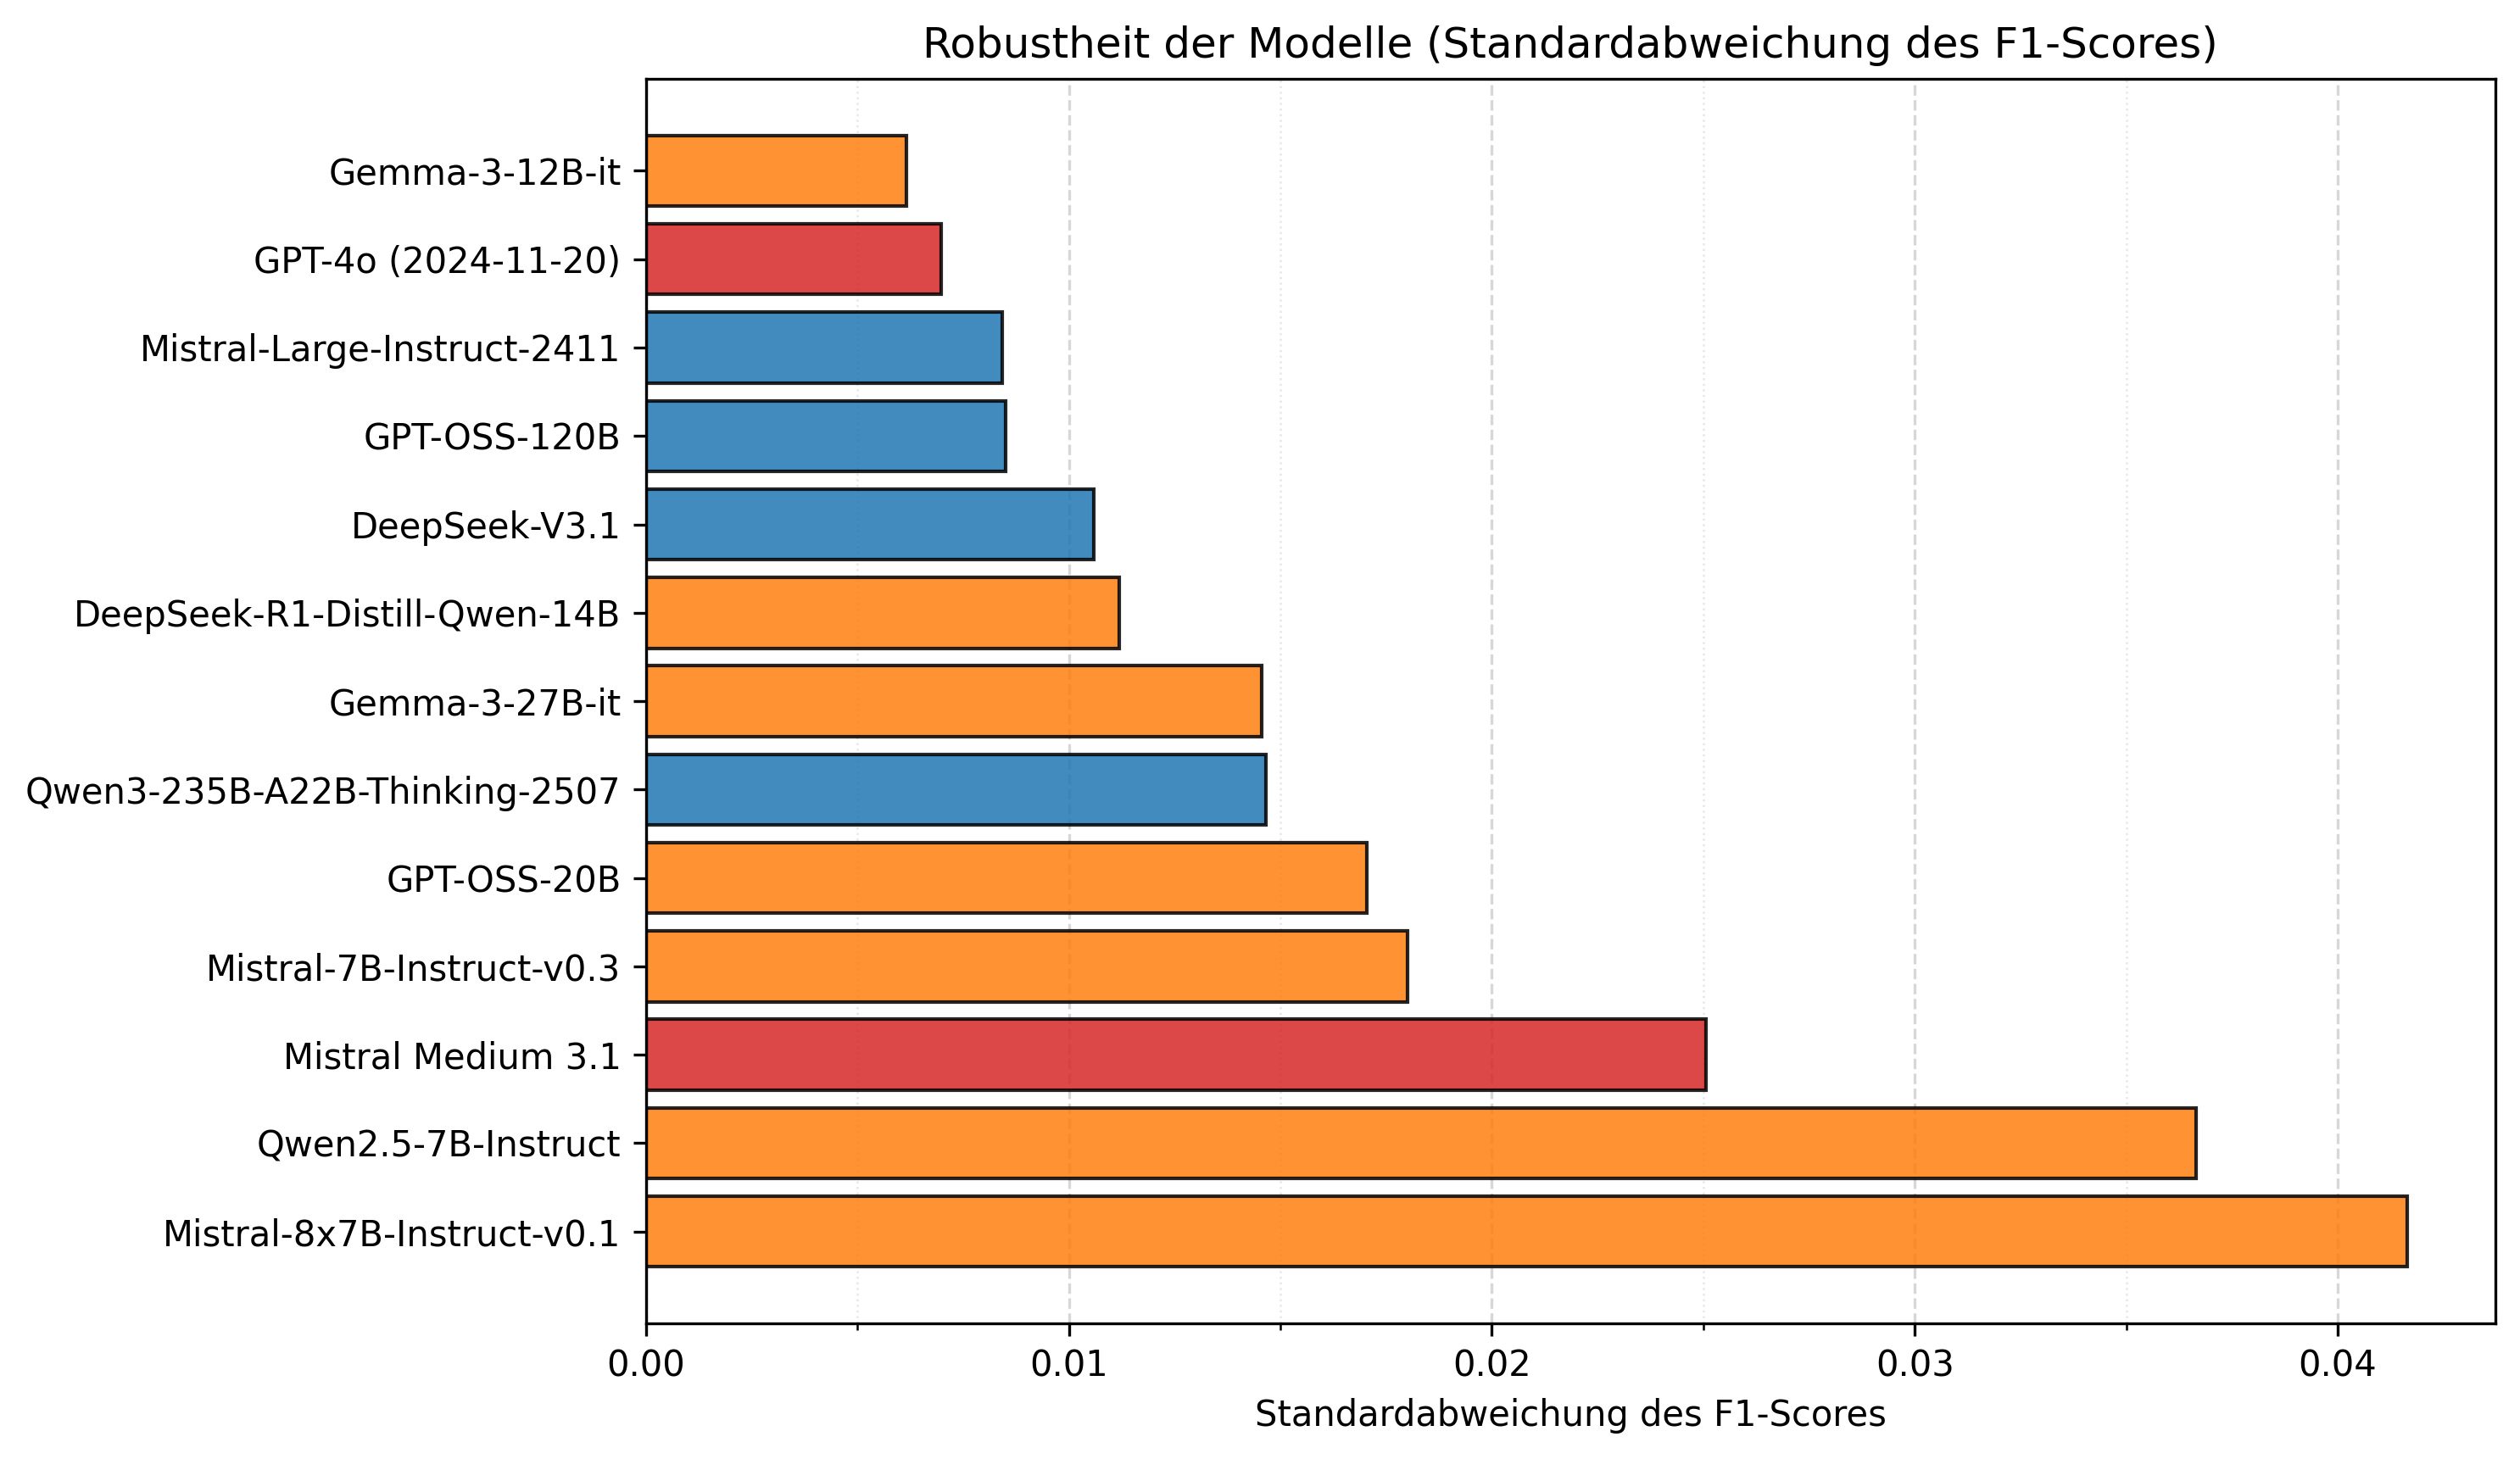
\includegraphics[width=\textwidth,trim=20 40 20 10,clip]{images/results/evaluation_robustness_f1_std}
    \caption{Robustheit der Modelle gemessen an der Standardabweichung des F1-Scores über alle Wiederholungen hinweg.}
    \label{fig:results-evaluation-robustness-f1-std}
\end{figure}

Abbildung \ref{fig:results-evaluation-robustness-f1-std} zeigt die Robustheit der Modelle gemessen an der Standardabweichung des F1-Scores über alle Wiederholungen hinweg. Hier zeigt sich eine große Varianz: Während einige Modelle wie \texttt{Gemma-3-12B.it} und \texttt{Mistral-Large-Instruct-2411} eine sehr geringe Standardabweichung von $\le 0{,}01$ aufweisen, zeigen andere Modelle wie \texttt{Mistral-8x7B-Instruct-v0.1} und \texttt{Qwen2.5-7B-Instruct} eine hohe Varianz von $\ge 0{,}03$ bis $\ge 0{,}04$ im F1-Score. Dies deutet darauf hin, dass die Leistung dieser Modelle stark von der Wahl des Seeds abhängen und ihre Leistung weniger stabil ist.